\clearpage

\section{cwTone}
\begin{tcolorbox}	
	\begin{tabular}{p{2.75cm} p{0.2cm} p{10.5cm}} 	
		\textbf{Header File}   &:& cwTone.h \\
		\textbf{Source File}   &:& cwTone.cpp \\
		\textbf{Version}       &:& 20180705 (\textbf{Student Name}: Romil Patel)
	\end{tabular}
\end{tcolorbox}

\subsection*{Input Parameters}

\textbf{frequency:} The frequency of CW tone depends on the bandwidth of the complex signal $I(t) + i\hspace{0.1cm}Q(t)$. The frequency of the signal should coincide to the right or left edge of the information carrying signal spectrum.
\\
\textbf{amplitude:} The amplitude of the signal should provide the Carrier to Signal Power Ratio (CSPR) of about $\sim$9dB.

\subsection*{Input Signals}
\textbf{Number}: 1, 2\\
\textbf{Type}: RealValue
\subsection*{Output Signals}
\textbf{Number}: 3, 4\\
\textbf{Type}: RealValue

\subsection*{Functional Description}
This block accepts two real valued signal, one is $I(t)$ and other $Q(t)$, and add a CW tone to both these signals. The tone added to both the signals are $90^o$ phase shifted to other. The signal output at port 3 and  4 can be written as $I(t)+A\cdot cos(2\pi Ft)$ and $I(t)+A\cdot sin(2\pi Ft)$, respectively. Where $A$ and $F$ represent the amplitude and frequency of the CW tone.  

\begin{figure}[h]
	\centering
	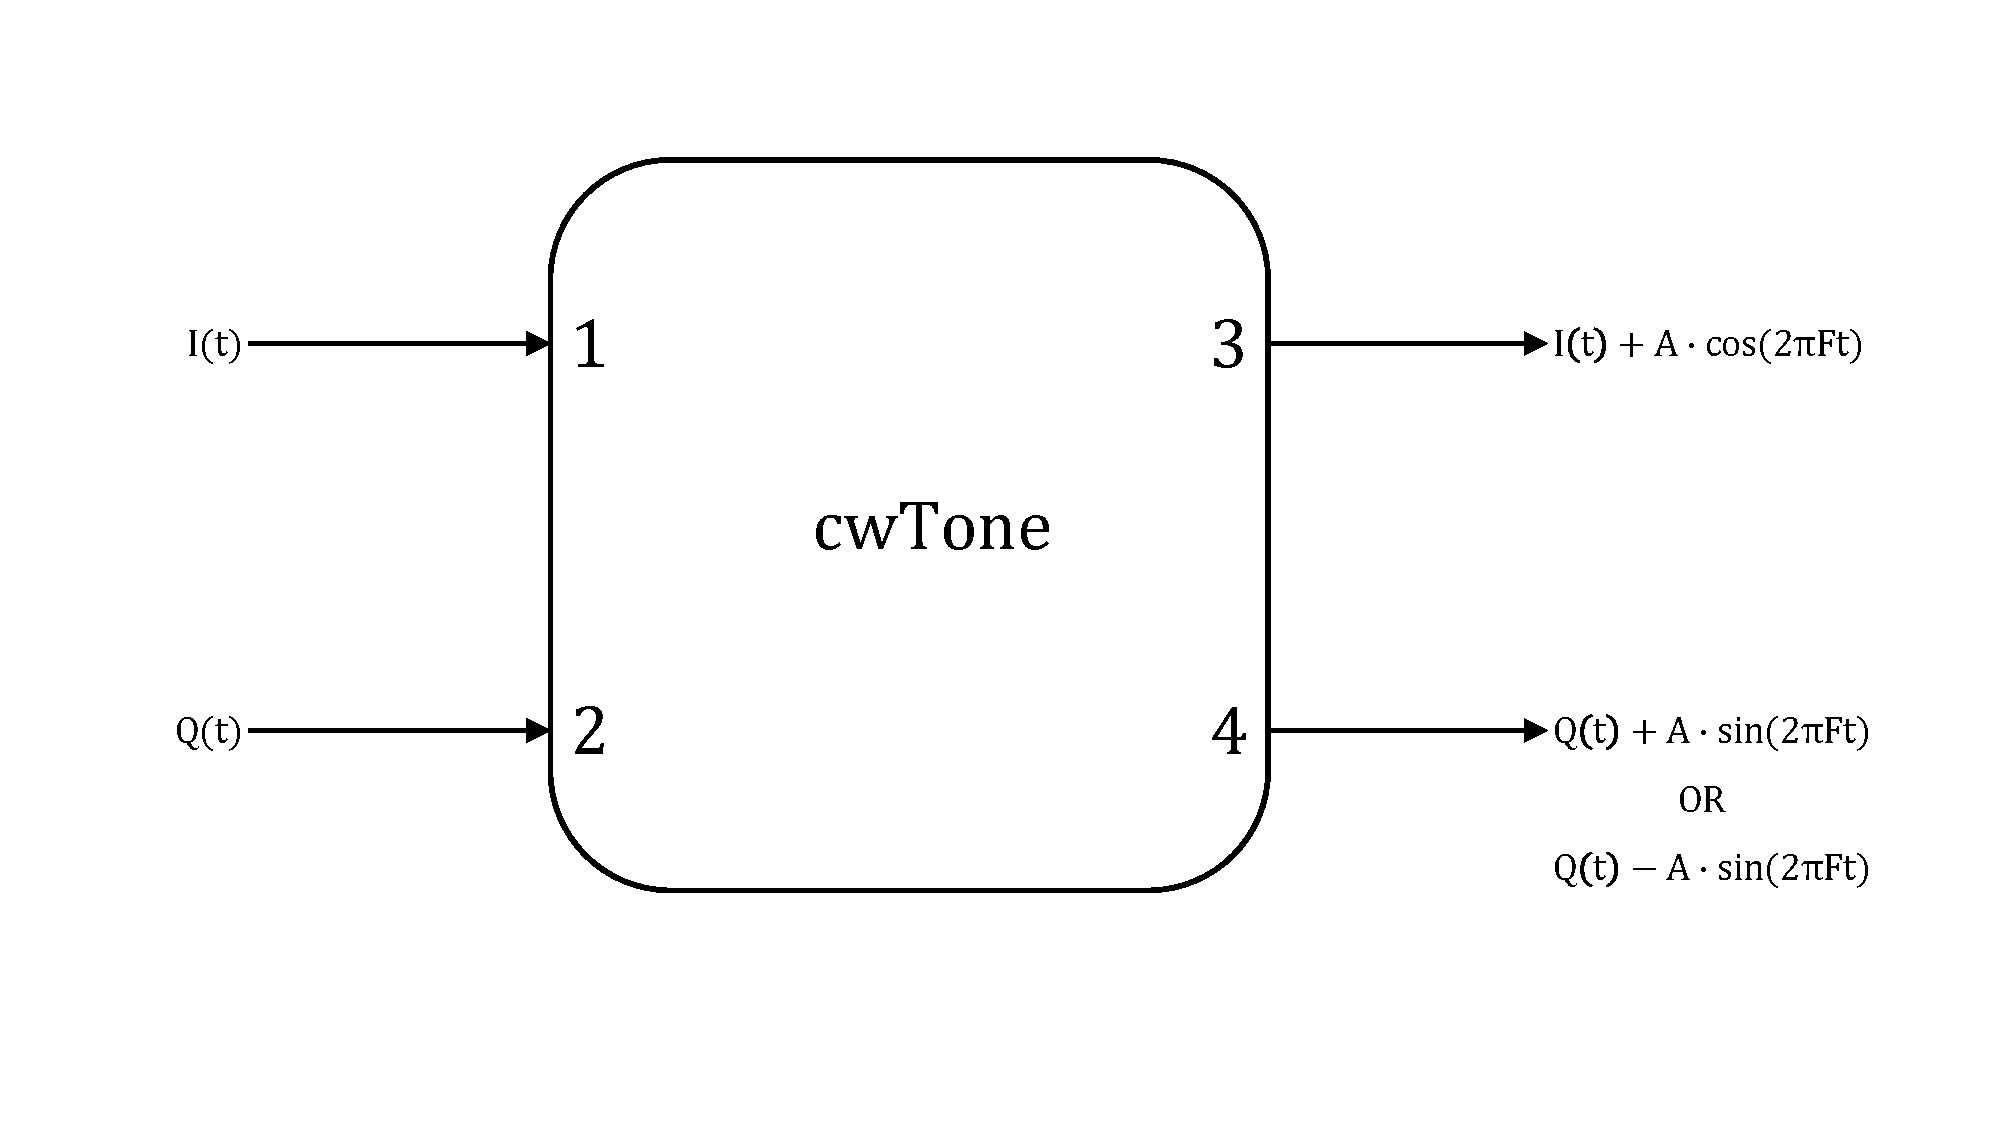
\includegraphics[width=0.6\textwidth, height=4cm]{./lib/cwTone/figures/cwTone.pdf}
	\caption{cwTone}\label{cwTOne}
\end{figure}